\section{Experiments} \label{sec:experiments}

We now present the empirical evaluation of these coresets.
We ran two kinds of experiments. On real-world data sets, we merely computed a coreset $\Omega$, followed by running $k$-means++ on $\Omega$. 
The $k$-means++ algorithm was repeated 5 times, each yielding a solution $\calS_i$, and as the best lower bound on the distortion we used the largest ratio $\max_i\left(\max\left(\frac{\cost_A(\calS_i)}{\cost_{\Omega}(\calS_i)},\frac{\cost_{\Omega}(\calS_i)}{\cost_A(\calS_i)}\right)\right)$.
For the benchmark, we used the evaluation as proposed in Section~\ref{sec:benchmark}. In addition, we also determined the distortion via simply running the $k$-means++ algorithm. 

Except for BICO, which is deterministic, this experiment was repeated for each coreset algorithm $10$ times. \omar{Experiments were repeated 10 times including BICO. Although vanilla BICO is deterministic, we used BICO with heuristic speed optimizations which are stochastic.} We aggregated the reported distortions by taking the maximum over all $10$ evaluations. In addition, we also preprocessed the data using the dimension reduction techniques described in Section~\ref{sec:algorithms}.


\subsection{Datasets}
To evaluate the behavior of different algorithms, we conducted experiments on 5 real-world datasets, as shown in~\cref{tab:real-world-datasets-overview}, in addition to our proposed benchmark.

% The real-world datasets include
% \textit{Census}\footnote{\url{https://archive.ics.uci.edu/ml/datasets/US+Census+Data+(1990)}},
% \textit{Covertype}\footnote{\url{https://archive.ics.uci.edu/ml/datasets/covertype}}, and 
% \textit{Tower}\footnote{\url{http://homepages.uni-paderborn.de/frahling/coremeans.html}}
% ---
% and several instances of the proposed benchmark.

The \textit{Census}\footnote{\url{https://archive.ics.uci.edu/ml/datasets/US+Census+Data+(1990)}} dataset is a small subset of the Public Use Microdata Samples from 1990 US census. It consists of demographic information encoded as 68 categorical attributes of 2,458,285 individuals. 

\textit{Covertype}\footnote{\url{https://archive.ics.uci.edu/ml/datasets/covertype}} is comprised of cartographic descriptions and forest cover type of four wilderness areas in the Roosevelt National Forest of Northern Colorado in the US. It consists of 581,012 records, 54 cartographic variables and one class variable. Although \textit{Covertype} was originally made for classification tasks, it is often used for clustering tasks by removing the class variable~\cite{AckermannMRSLS12}.

\textit{Tower}\footnote{\url{http://homepages.uni-paderborn.de/frahling/coremeans.html}} is a 2,560 by 1,920 picture of a tower on a hill where each pixel is represented by a RGB color value. This dataset consists of 4,915,200 rows and 3 columns. 
We used the datasets \textit{Census}, \textit{Covertype} and \textit{Tower} as these are often used to evaluate the performance of coreset algorithms. 

To include larger datasets in evaluation, we used \textit{Caltech} and \textit{NYTimes}. \textit{Caltech} was inspired by~\cite{FGSSS13}. It was created by computing SIFT features from the images in the Caltech101 dataset\footnote{\url{http://www.vision.caltech.edu/Image_Datasets/Caltech101/}}. This database contains pictures of objects partitioned into 101 categories. Disregarding the categories, we concatenated the 128-dimensional SIFT vectors from each image into one large data matrix. 
We decided to include the \textit{NYTimes}\footnote{\url{https://archive.ics.uci.edu/ml/datasets/bag+of+words}} dataset in our experiments as the number of dimensions is very large. \textit{NYTimes} is composed of the word counts of 300,000 news articles from The New York Times. The vocabulary size of the text collection is 102,660.

To understand how denoising effects the quality of the coreset outputs, we applied Principal Component Analysis (PCA) on \textit{Caltech}, \textit{Census} and \textit{Covertype} by computing the $k$ singular vectors corresponding to the largest singular values. For these three datasets, we preserve the dimensions of the original datasets. For the \textit{NYTimes} dataset, we experimented with both PCA and terminal embeddings to reduce the number of dimensions.

As for the benchmark dataset, instances were generated to roughly match the sizes of the real-world datasets. The chosen parameters values and the corresponding dataset sizes are shown in ~\cref{tab:benchmark-instances-overview}. 
% We generated a set of instances with no scaling i.e., $\beta=1.0$ (referred to as \textit{Benchmark-1.0}) and with maximum scaling; $\beta = 2.0$ (\textit{Benchmark-2.0}).




%
\begin{table}
	\begin{center}%\centering
	\caption{The sizes of the real-world datasets used for the experimental evaluation}
	\label{tab:real-world-datasets-overview}
% 	\resizebox{\textwidth}{!}{
	\begin{tabular}{lrr}
		\toprule
        
		    & Data points
		    & Dimensions
            \\
		\midrule
		\textit{Caltech}
    		& 3,680,458
    		& 128
    		\\
		\textit{Census}
    		& 2,458,285
    		& 68
    		\\
	    \textit{Covertype}
    	    & 581,012
    		& 54
    		\\
	    \textit{NYTimes}
    	    & 500,000
    		& 102,660
    		\\
        \textit{Tower}
            & 4,915,200
    		& 3
    		\\
		\bottomrule
	\end{tabular}\\
	\end{center}
% 	}
\end{table}



%
\begin{table}
	\begin{center}%\centering
	\caption{The parameter values and the sizes of the benchmark instances used for the experimental evaluation.}
	\label{tab:benchmark-instances-overview}
% 	\resizebox{\textwidth}{!}{
	\begin{tabular}{rrrr}
		\toprule
        $k$
		    & $\alpha$
		    & Data points
		    & Dimensions
            \\
		\midrule
        10
    		& 6
    		& 1,000,000
    		& 60
    		\\
        20
    		& 5
    		& 3,200,000
    		& 100
    		\\
        30
    		& 4
    		& 810,000
    		& 120
    		\\
        40
    		& 4
    		& 2,560,000
    		& 160
    		\\
    %     50
    % 		& 4
    % 		& 6,250,000
    % 		& 200
    % 		\\
		\bottomrule
	\end{tabular}\\
	\end{center}
% 	}
\end{table}

\subsection{Algorithm Parameters}
We followed the same experimental procedure with respect to the choice of parameter values for the algorithms as prior works~\cite{AckermannMRSLS12, FGSSS13}. For the target coreset size, we used $200k$ for all our experiments. On \textit{Caltech}, \textit{Census},  \textit{Covertype} and \textit{NYTimes}, we used $k$ values in $\{10, 20, 30, 40, 50\}$, while for \textit{Tower} we used larger cluster sizes $k \in \{20, 40, 60, 80, 100\}$. On the benchmark instances, we settled on $k \in \{10, 20, 30, 40\}$ as a reasonable trade-off between running time and dataset size.



\subsection{Setup}
We implemented Sensitivity Sampling, Group Sampling, Ray Maker, and StreamKM++ in C++. The source code can be found on GitHub\footnote{Link to repository will be provided later.}. For BICO, we used the authors' reference implementation\footnote{\url{https://ls2-www.cs.tu-dortmund.de/grav/en/bico}}. The source code was compiled with gcc 9.3.0. The experiments were performed on a machine with 14 cores (3.3 GHz) and 256 GB of memory.

\subsection{Results}

\begin{figure*}
  \caption{The distortions of the evaluated algorithms on 5 real-world datasets and on the proposed benchmark. Lower bar is better.}
  \label{fig:distortions}
  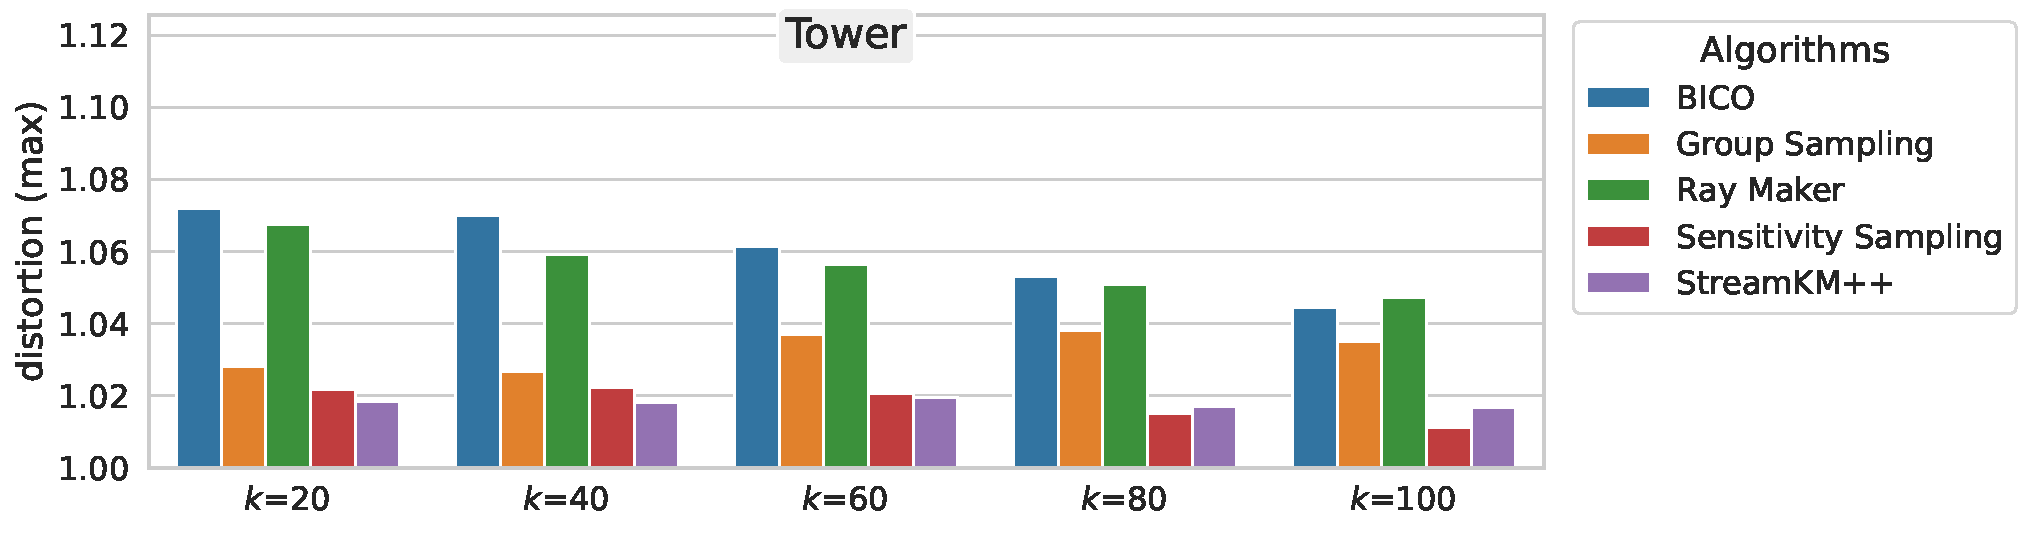
\includegraphics[width=.65\linewidth]{figures/distortions-Tower.pdf}
  \newline \newline
  \subfloat{
    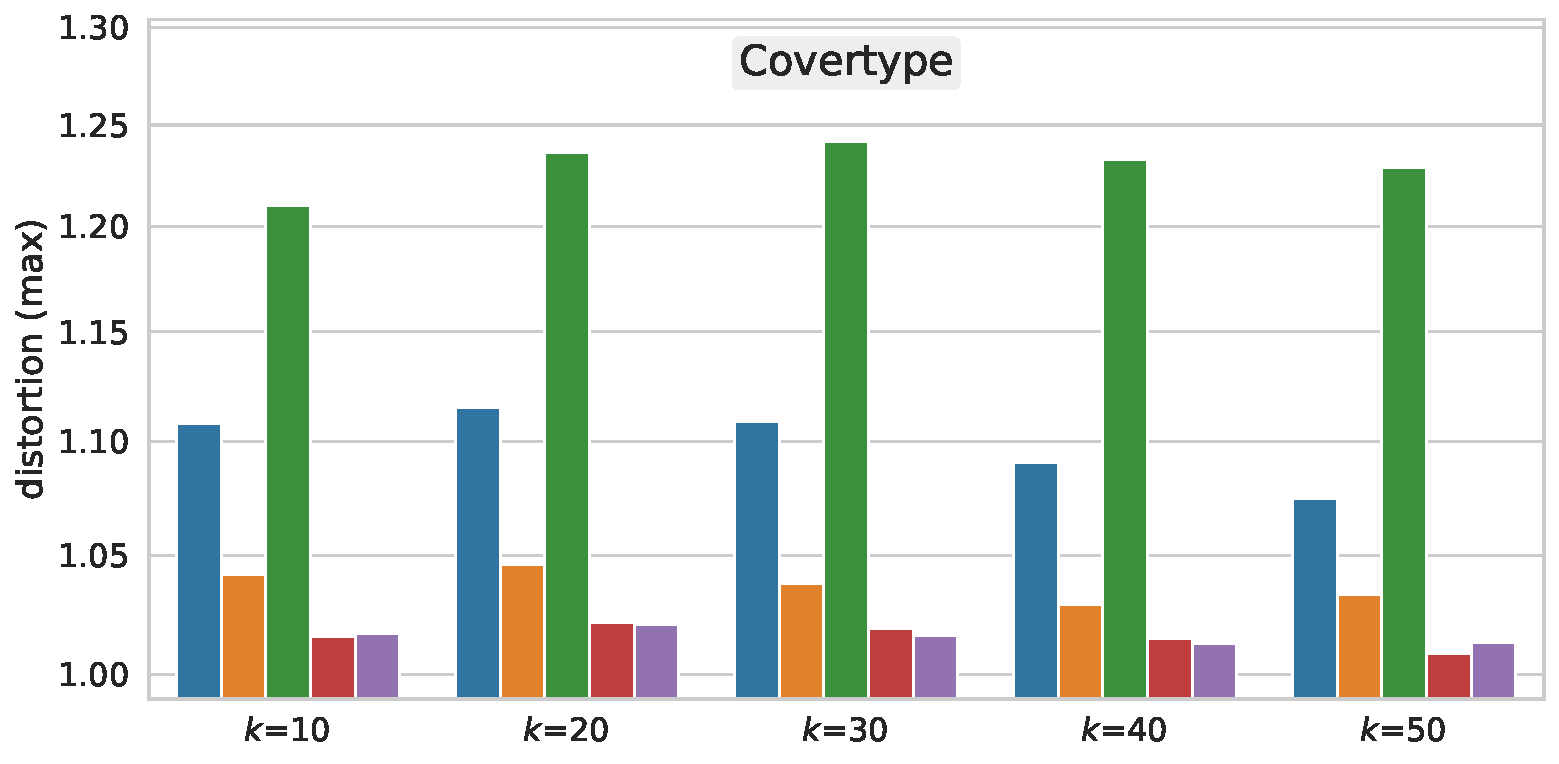
\includegraphics[width=0.5\textwidth]{figures/distortions-Covertype.pdf}
  }
  \subfloat{
    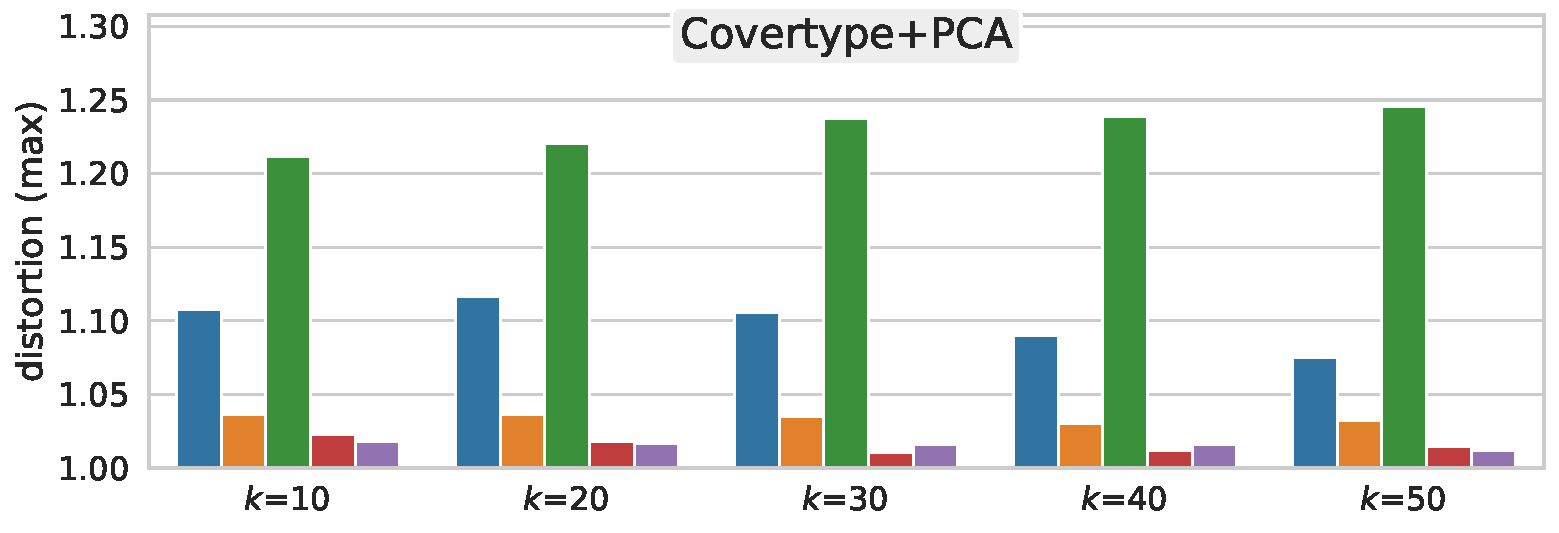
\includegraphics[width=.5\linewidth]{figures/distortions-Covertype+PCA.pdf}
  }
  \newline \newline
  \subfloat{
    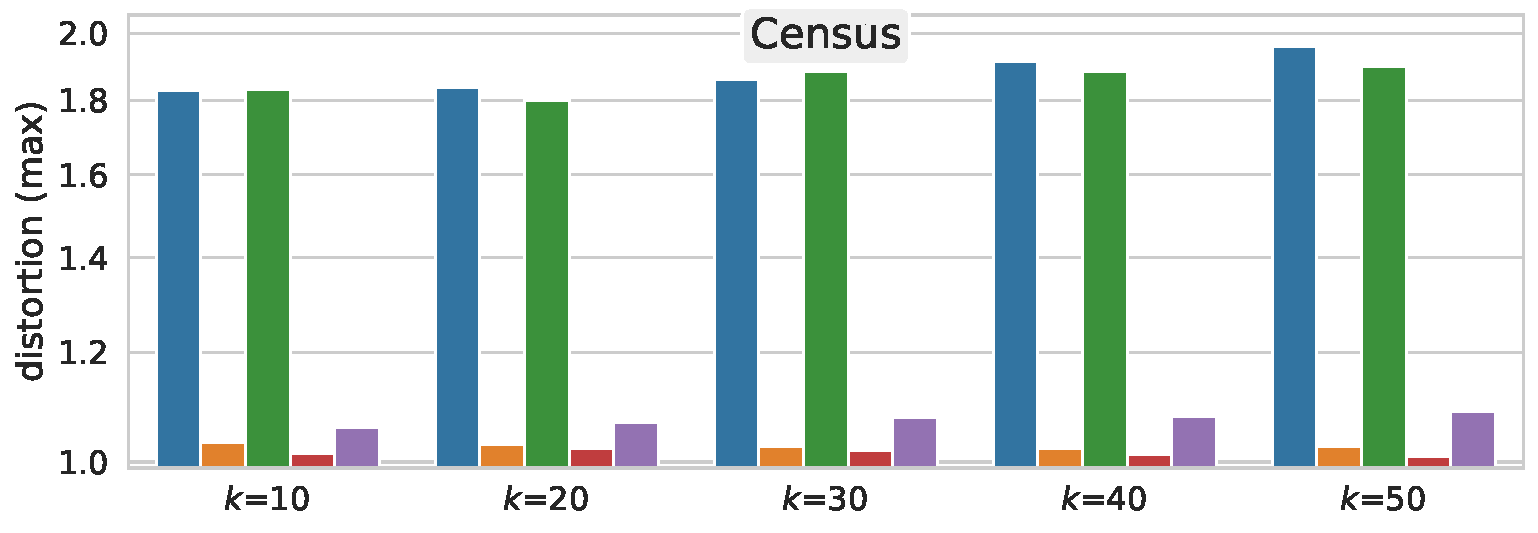
\includegraphics[width=0.5\textwidth]{figures/distortions-Census.pdf}
  }
  \subfloat{
    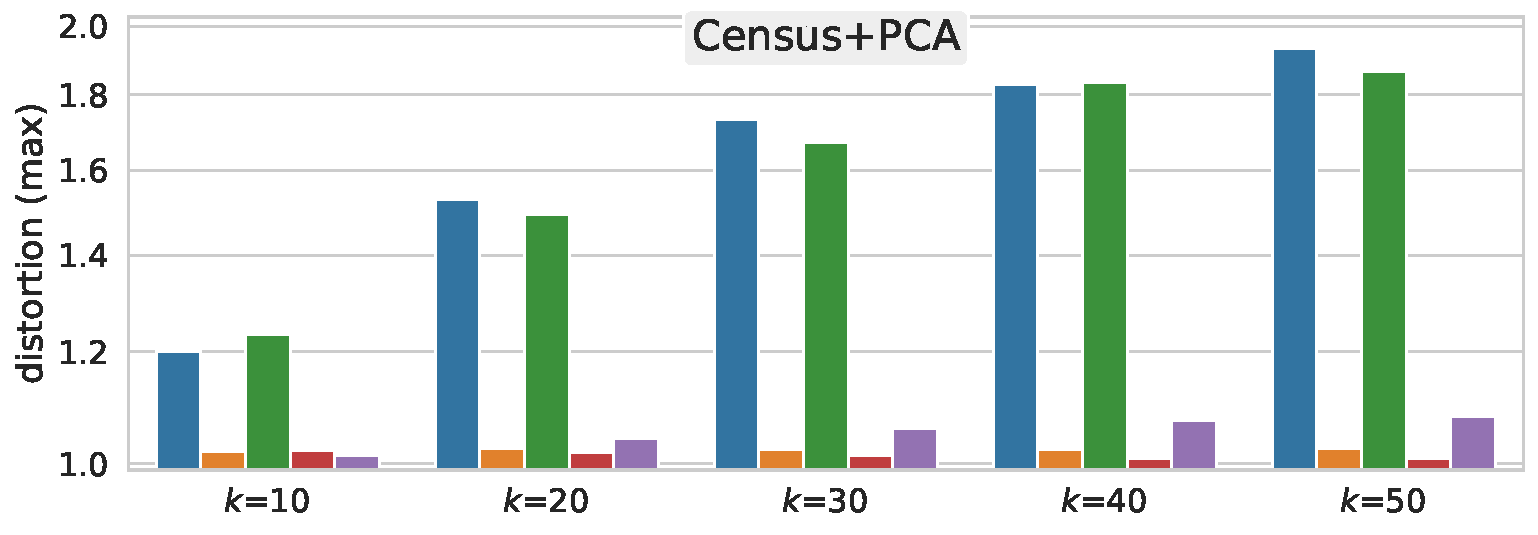
\includegraphics[width=.5\linewidth]{figures/distortions-Census+PCA.pdf}
  }
  \newline \newline
  \subfloat{
    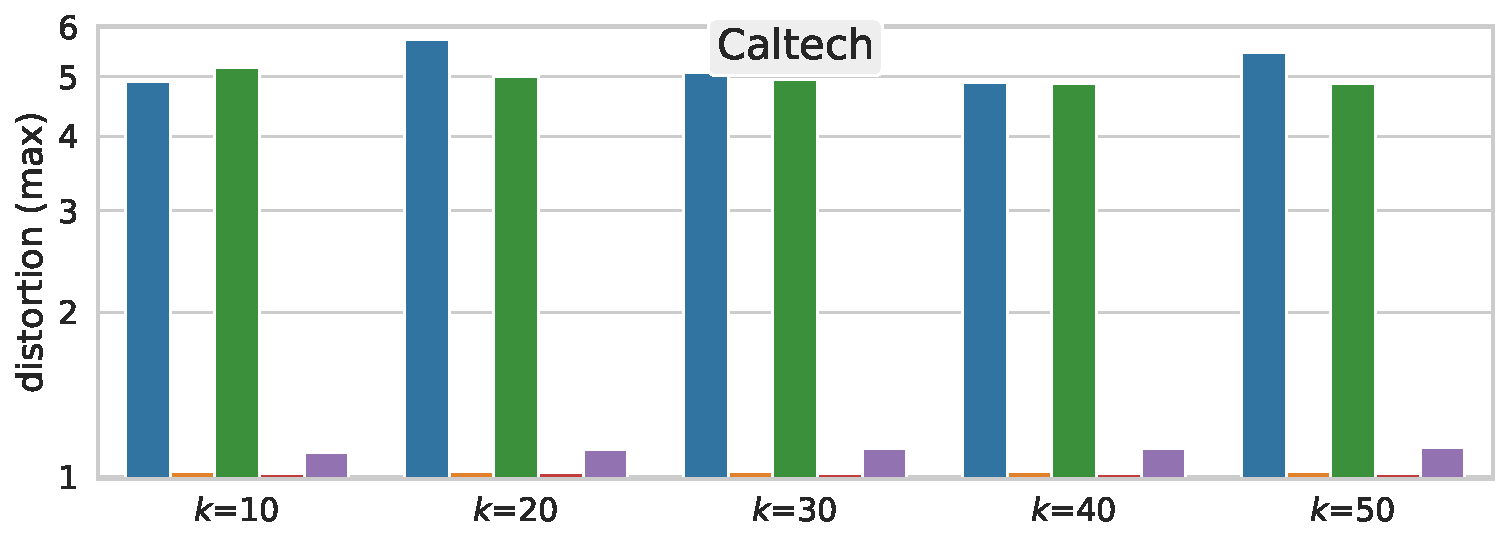
\includegraphics[width=0.5\textwidth]{figures/distortions-Caltech.pdf}
  }
  \subfloat{
    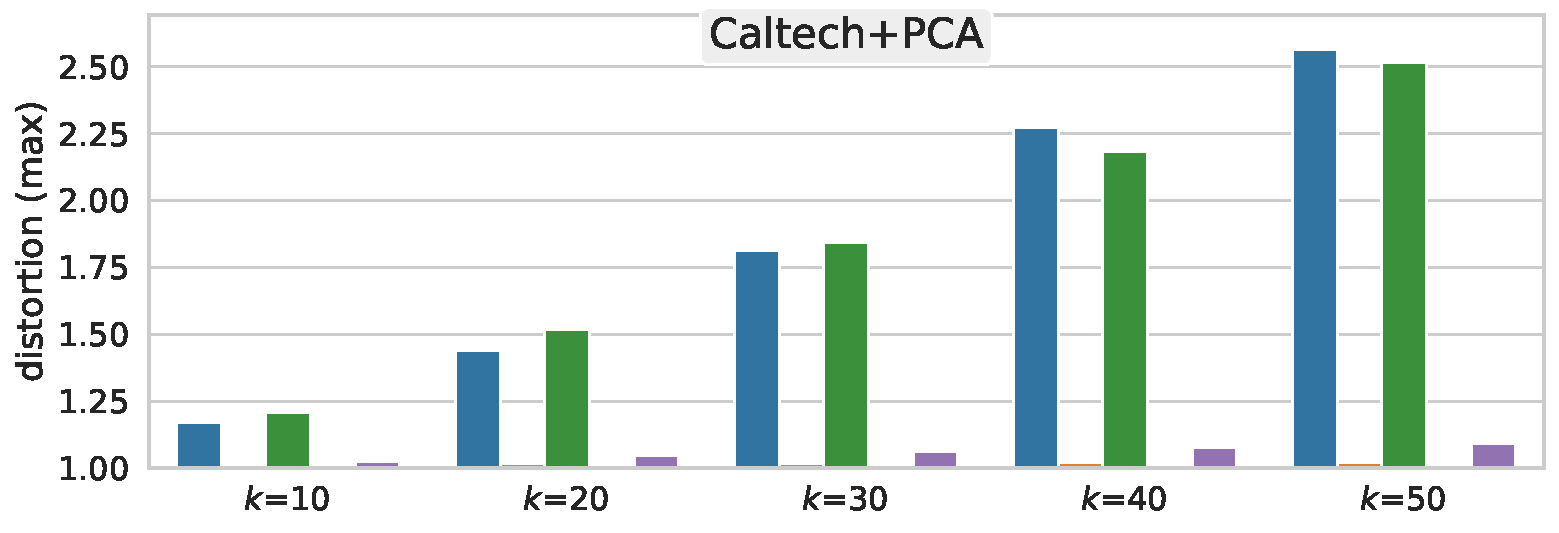
\includegraphics[width=.5\linewidth]{figures/distortions-Caltech+PCA.pdf}
  }
  \newline \newline
  \subfloat{
    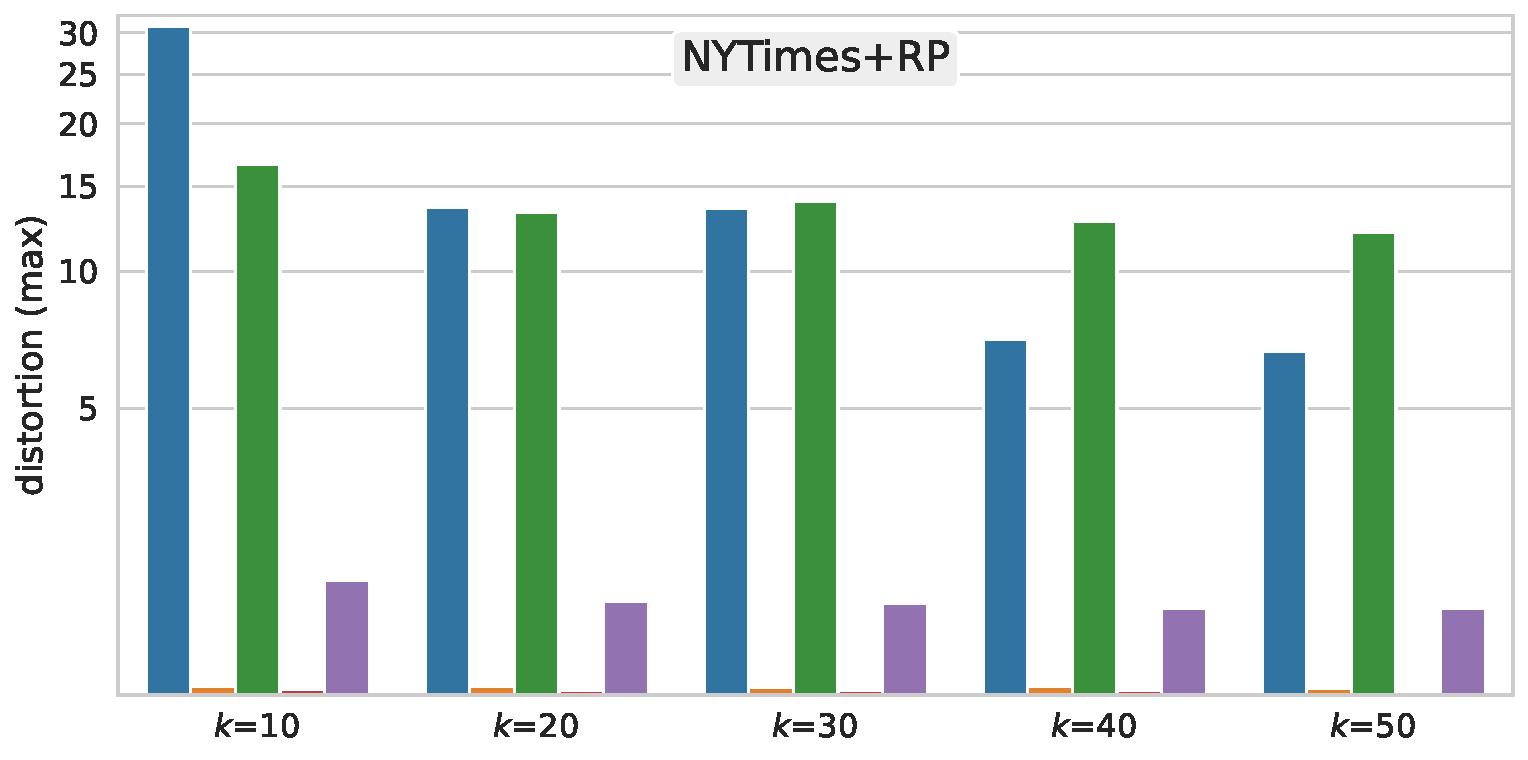
\includegraphics[width=0.5\textwidth]{figures/distortions-NYTimes+RP.pdf}
  }
  \subfloat{
    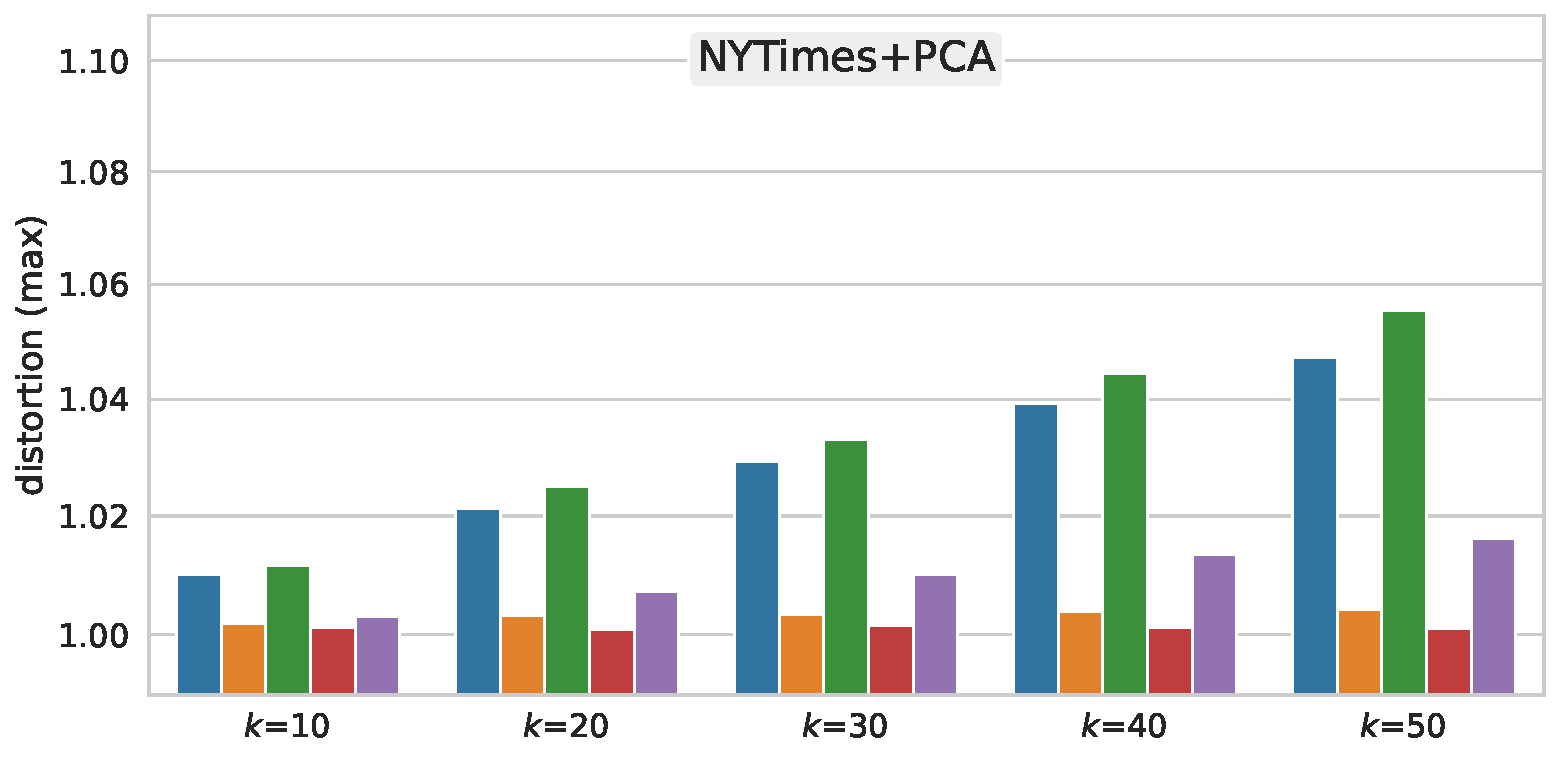
\includegraphics[width=.5\linewidth]{figures/distortions-NYTimes+PCA.pdf}
  }
  \newline \newline
  \subfloat{
    \\[1ex]
    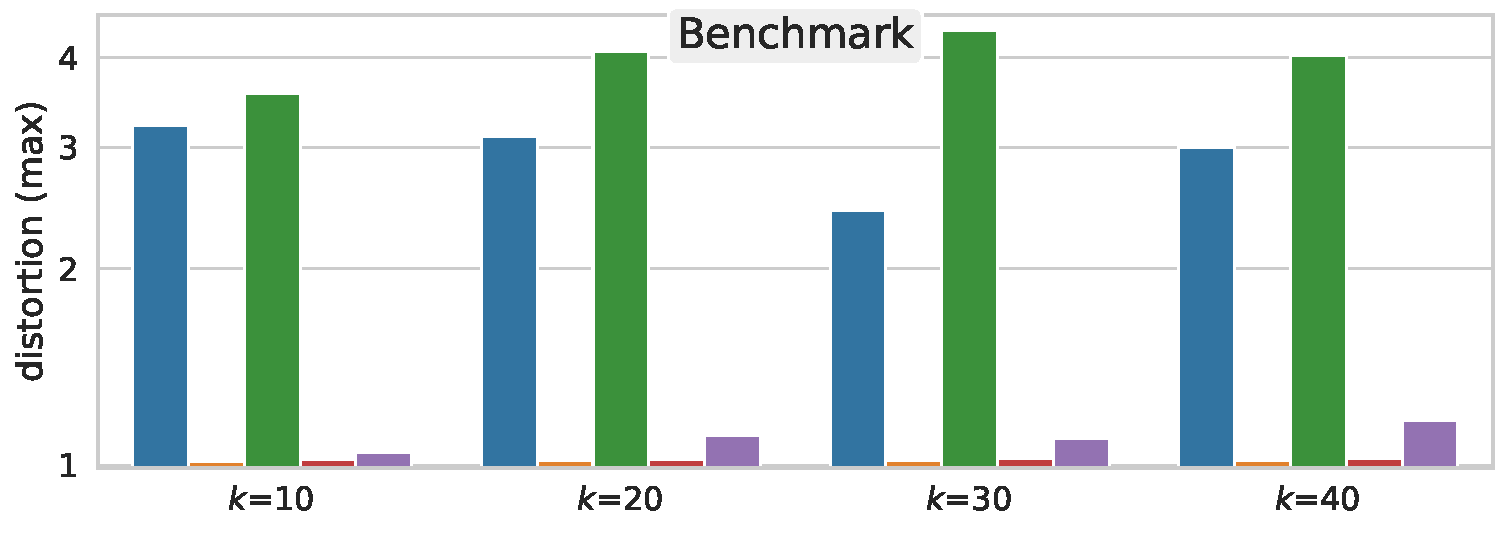
\includegraphics[width=0.5\textwidth]{figures/distortions-Benchmark.pdf}
  }
  \subfloat{
    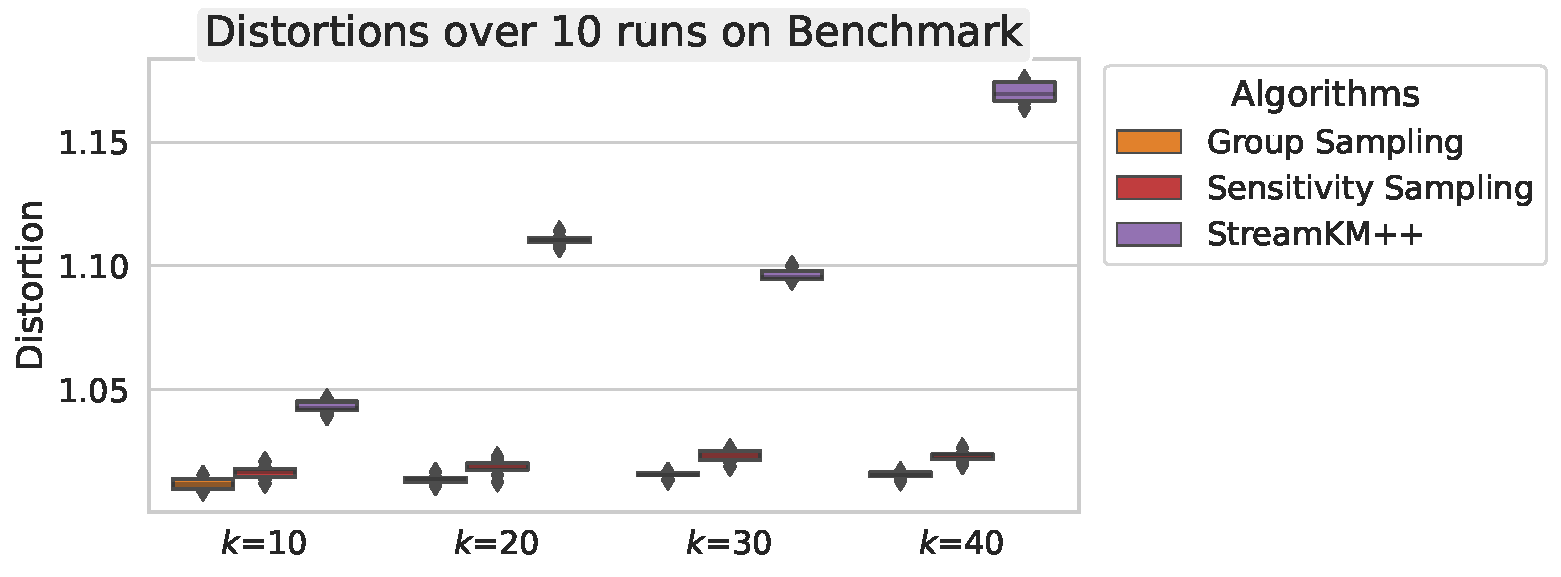
\includegraphics[width=.5\linewidth]{figures/boxplot-Benchmark-GS-SS-StreamKM.pdf}
  }
  
\end{figure*}

We summarized the results in \cref{fig:distortions}.
All five algorithms are matched on the \textit{Tower} dataset. The worst distortions across the algorithms are close to 1, and performance between the algorithms is negligible. \textit{Tower} is a simple dataset with very low dimensionality ($d=3$). The performance difference between sampling-based and movement-based methods become more pronounced as the number of dimensions increase. On \textit{Covertype} with its 54 features, Ray Maker performs the worst followed by BICO. The performance does not change much despite reducing noise with PCA. Differences in performance are more stark on \textit{Census} and \textit{Caltech} where methods based on importance sampling are better. For \textit{Census} ($d=68$), the preprocessing step with PCA improves the performance of BICO and Ray Maker slightly for lower values of $k$. The distortions of BICO and Ray Maker are reduced markedly on \textit{Caltech} ($d=128$) after applying PCA. We observe that BICO and Ray Maker have very large distortions on \textit{NYTimes} when random projections are used for dimensionality reduction. On the \textit{Benchmark} dataset, Ray Maker is the worst while Sensitivty Sampling and Group Sampling are the best. StreamKM++ performs also very well compared to BICO.
